% !TEX root = thesis.tex
\chapter{Towards Efficient Inference: Techniques and Solutions}\label{chap:methods}

Building upon the previous chapter, this chapter systematically surveys the techniques that have been developed to reduce the resource demands of \ac{llm} inference. For each technique the discussion covers its core mechanism, the bottleneck it addresses, its accuracy--efficiency trade-off, and its practical implications for edge deployment. In~\ref{tab:bottleneck-technique-map} the principal inference bottlenecks identified in Chapter~2 are mapped to the optimisation techniques discussed in this chapter. Since several methods address more than one resource constraint, the categories are not mutually exclusive.

\begin{table}[h]
    \renewcommand{\arraystretch}{1.25}
    \begin{tabularx}{\textwidth}{
        >{\raggedright\arraybackslash}p{0.24\textwidth}
        >{\raggedright\arraybackslash}p{0.34\textwidth}
        >{\raggedright\arraybackslash}X
    }
        \toprule
        \textbf{Inference bottleneck}
        & \textbf{Relevant techniques}
        & \textbf{Primary effect} \\
        \midrule

        Weight memory and memory bandwidth
        & Weight quantisation(~\ref{sec:quantization}), pruning~\ref{sec:pruning}, knowledge distillation~\ref{sec:knowledge-distillation}
        & Reduces the model size and the amount of weight data transferred
        from memory during inference. \\

        \addlinespace

        KV-cache memory
        & KV-cache quantisation~\ref{subsubsection:kv-cache-quantization}, PagedAttention~\ref{subsubsection:pagedattention}, knowledge distillation~\ref{subsubsection:knowledge-distillation}
        & Reduces the size of the KV cache or improves how its memory is
        allocated and managed. \\

        \addlinespace

        Attention computation and memory traffic
        & FlashAttention~\ref{subsubsection:flashattention}, pruning~\ref{subsubsection:pruning}
        & Reduces attention-related memory accesses, intermediate storage,
        or arithmetic operations. \\

        \addlinespace

        Sequential autoregressive decoding
        & Speculative decoding~\ref{subsubsection:speculative-decoding}
        & Allows multiple candidate tokens to be verified in one target-model
        forward pass, reducing the number of sequential decoding steps. \\

        \addlinespace

        Low hardware utilisation
        & Continuous batching~\ref{subsubsection:continuous-batching}, PagedAttention~\ref{subsubsection:pagedattention}
        & Improves accelerator utilisation by dynamically grouping requests
        and using memory more efficiently. \\

        \addlinespace

        Hardware portability and kernel efficiency
        & llama.cpp~ref{subsubsection:llama-cpp}, MLC-LLM~ref{subsubsection:mlc-llm}, vLLM~ref{subsubsection:vllm}
        & Provides hardware-specific kernels, runtime optimisations, and
        memory-management strategies for different deployment platforms. \\

        \bottomrule
    \end{tabularx}

    \centering
    \caption{Mapping of major LLM inference bottlenecks to the efficiency
    techniques that address them.}
    \label{tab:bottleneck-technique-map}
\end{table}


\section{Model Compression}\label{sec:model-level}

Model compression techniques reduce the size of the model itself shrinking weight memory and, consequently, the bandwidth required to load those weights during each decode step. They are pre-deployment operations and impose a one-time cost in compute or data for calibration.

\subsection{Quantization}\label{sec:quantization}

Quantization is a model-compression strategy that lowers the numerical precision of model parameters and/or intermediate values. Instead of storing and computing with high-precision formats such as FP32, FP16 or BF16, quantized models use lower-bit formats such as INT8, INT4, or even lower representations. This is especially useful for edge deployment, where memory capacity, bandwidth, energy consumption, and computational resources are limited. However, quantizing large language models is more difficult than quantizing many conventional neural networks because Transformer architectures contain attention layers, high-dimensional hidden states, and activation distributions with large dynamic ranges. These properties make LLMs sensitive to numerical approximation, so aggressive quantization can reduce model quality if it is not carefully controlled. \cite{yue2024reviewonedge}

Quantization methods can be classified according to when quantization is introduced and which tensors are quantized. Post Training Quantization(PTQ) modifies an already trained model, and requires retraining which can be very costly, whereas \ac{qat} incorporates simulated quantization during training or fine-tuning. Independently, a method may quantize only the weights or both weights and activations \cite{zhou2024efficientinf}.


\subsubsection{Weight-only quantization}\label{weight-only-quantization}

In weight-only quantization the precision of the model’s stored parameters (weights) are reduced while usually keeping activations in higher precision. This mainly lowers memory usage and can improve inference efficiency. Examples include LLM.int8(), which uses vectorwise quantization and mixed-precision decomposition enabling Int8 matrix multiplication for feed-forward and attention projection layers in transformers. This has been shown to have minimal precision loss and maintain performance for models with upto 175B parameters \cite{dettmers2022llm}. Another method known as GPTQ takes compression even further by reducing the bitwidth down to 3 or 4 bits per weight for models with up to 175B parameters without significant accuracy loss. This method uses approximated second-order information which allows it to identify sensitive weights and compensate for quantization errors by adjusting the remaining weights \cite{frantar2023gptq}.

\subsubsection{Weight-activation (co-)quantization}\label{weight-activation-quantization}

Weight-activation (co-)quantization goes further by reducing the precision of both weights and intermediate activations. This can provide additional memory and computational savings, but it is harder because activations in LLMs often contain large outliers and irregular value ranges. Methods such as ZeroQuant and SmoothQuant address this by using more refined scaling or grouping strategies. In particular, SmoothQuant shifts part of the quantization difficulty from activations to weights through mathematically equivalent scaling transformations, enabling efficient 8-bit weight-and-activation quantization with limited accuracy loss.  \cite{yue2024reviewonedge}



\subsection{Pruning}\label{sec:pruning}

Pruning removes parameters from the model that contribute least to its predictions in accordance with some pruning criterion such as minimising the reconstruction loss of the model \cite{zhou2024efficientinf}. This in turn brings about a reduction in both weight memory and \ac{flops} count. The two principal strategies: \emph{unstructured} and \emph{structured} pruning differ in \emph{what} they remove and, consequently, in the hardware speedup they deliver.illustrates both approaches. Unstructured pruning sets individual weights to zero while preserving
the original tensor dimensions. Consequently, the reduction in the
number of non-zero parameters does not automatically produce a
proportional reduction in inference latency. Practical acceleration
depends on sparse storage formats, sparse-aware kernels, and compatible
hardware support. Structured pruning instead removes complete regular
structures, such as rows, columns, attention heads, or hidden
dimensions, thereby producing smaller dense operations that can
generally be executed using conventional dense linear-algebra
kernels~\cite{frantar2022spdy,wang2019structured}.


\subsubsection{Unstructured pruning}\label{unstructured-pruning} 

Unstructured pruning removes or sets individual scalar weights to zero, producing an irregular sparsity pattern while retaining the original tensor dimensions. SparseGPT is a one-shot post-training example of an unstructured pruning method designed for
large-scale generative language models. The method was evaluated on
models including OPT-175B and BLOOM-176B and was able to reach
50--60\% unstructured sparsity without retraining. At 60\% sparsity,
the authors report only a small increase in language-model perplexity,
while the pruning procedure required less than 4.5 hours for the
largest evaluated models~\cite{frantar2023sparsegpt}. These results
show that a large proportion of individual weights can be removed
without substantially degrading predictive quality. However, the
reported sparsity does not by itself imply an equivalent reduction in
inference latency, since practical acceleration depends on sparse
storage formats, sparse-aware kernels, and suitable hardware support. 

\subsubsection{Structured pruning}\label{structured-pruning} 

Structured pruning removes entire, regular sub-structures such as rows or columns of weight matrices, attention heads, \ac{ffn} intermediate dimensions, or whole Transformer layers yielding a strictly smaller \emph{dense} matrix that requires no sparse encoding and executes efficiently on any standard hardware. LLM-Pruner removes coupled structures, such as groups of channels,
using gradient-based importance estimates. On Vicuna-7B, pruning
approximately 20\% of the parameters retained about 92\% of the
original model's average zero-shot performance across the evaluated
classification benchmarks~\cite{ma2023llmpruner}. The method also
supports performance recovery through LoRA-based post-training using
50\,000 training samples, which the authors report can be completed in
approximately three hours. At substantially higher pruning ratios,
however, the performance degradation becomes considerably larger,
indicating that structured pruning offers direct reductions in dense
model size and computation at the cost of a stronger
compression--accuracy trade-off.

The reported results should be interpreted with care because the two
methods use different pruning structures and evaluation metrics.
SparseGPT primarily reports the effect of unstructured sparsity on
language-model perplexity, whereas LLM-Pruner evaluates structured
parameter removal using average downstream-task performance.
Consequently, the reported percentages are not directly comparable.

% ============================================================
%  Unstructured vs. Structured Pruning
% ============================================================
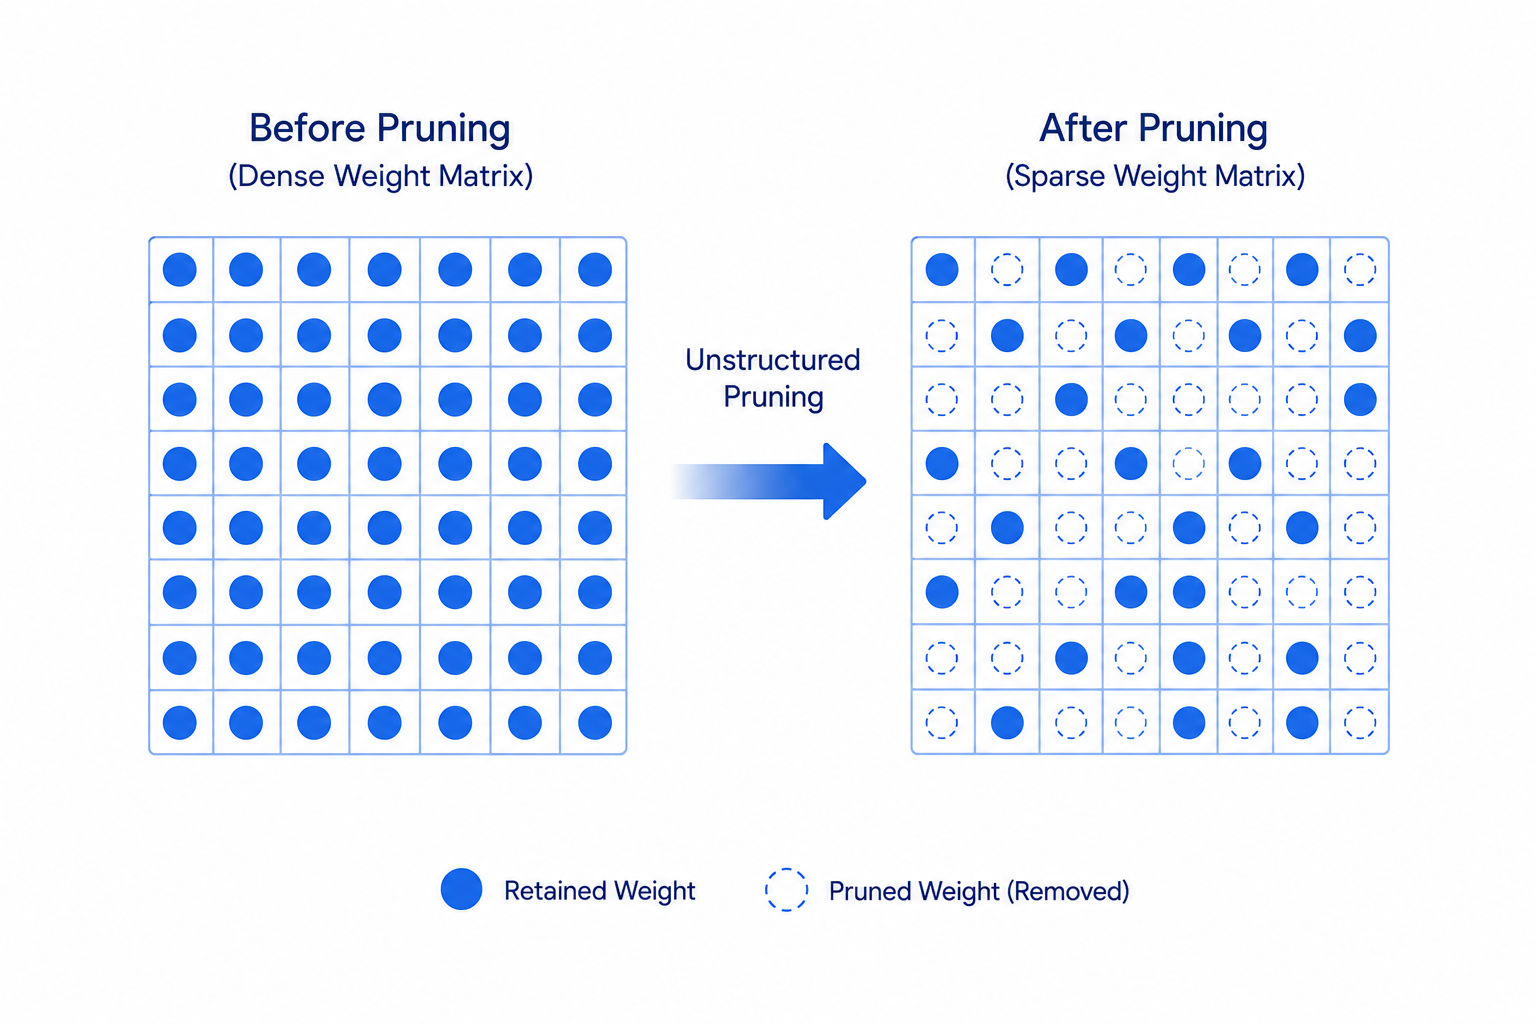
\includegraphics[width=0.5\textwidth]{figures/unstructure-pruning.png}
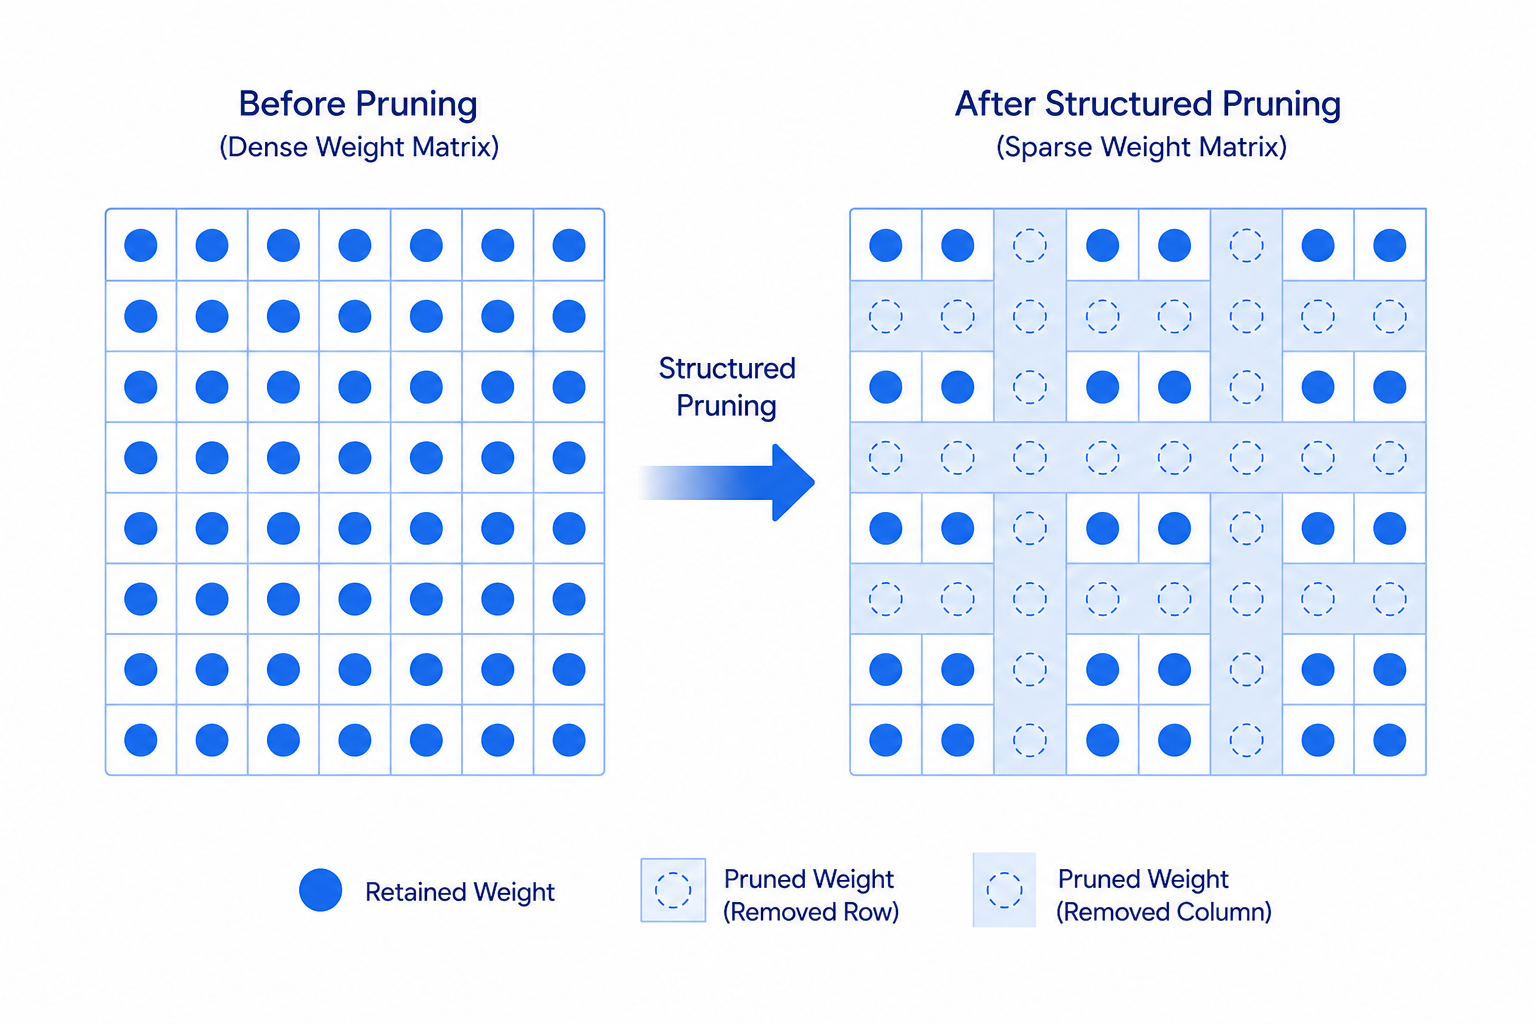
\includegraphics[width=0.5\textwidth]{figures/structured-pruning.png}


\subsection{Knowledge Distillation}\label{sec:distillation}

Knowledge Distillation (\acs{kd}) is a model compression technique in which a smaller student model is trained to imitate the behavior of a larger teacher model. In the context of large language models, KD is used to transfer knowledge and capabilities from powerful LLMs into smaller language models, reducing memory and computational requirements while preserving as much performance as possible. KD methods for LLMs are commonly divided into white-box and black-box approaches. \cite{zhou2024efficientinf}

\paragraph{White-box knowledge distillation.}
White-box knowledge distillation assumes access to the internal output
distribution or intermediate representations of the teacher model.
A representative example is MiniLLM, which distils an accessible
large language model into a smaller generative model using the
teacher's token-level probability distribution. Unlike conventional
knowledge distillation, which commonly minimises the forward
Kullback--Leibler divergence, MiniLLM employs the reverse
Kullback--Leibler divergence. This objective discourages the student
from assigning probability mass to low-probability regions of the
teacher distribution and was found to improve response quality,
calibration, and long-text generation. The method was evaluated across
teacher and student models ranging from 120 million to 13 billion
parameters~\cite{gu2024minillm}.

\paragraph{Black-box knowledge distillation.}
Black-box knowledge distillation is used when the teacher's parameters,
hidden states, and output logits are unavailable. In this setting, the
teacher is accessed only through its generated responses. Distilling
Step-by-Step is a representative method in which a large language
model is prompted to generate both task labels and natural-language
rationales for training examples. These outputs are then used as
additional supervision in a multi-task objective for a smaller student
model. The rationales provide intermediate task knowledge that is not
contained in the final label alone, allowing the student to learn with
less training data. In the reported experiments, a 770-million-parameter
T5 student outperformed a few-shot-prompted 540-billion-parameter PaLM
model on one benchmark while using only 80\% of the available training
data~\cite{hsieh2023distilling}.

The principal distinction is therefore the information available from
the teacher. White-box methods can directly align the student's
probability distribution or internal representations with those of the
teacher, but require access to the teacher model. Black-box methods are
applicable to proprietary models exposed through an API, although the
student can learn only from the text, labels, or rationales generated
by the teacher.



\section{Inference-Level Optimisations}\label{sec:inference_opts}

These techniques modify the attention mechanism or the \ac{kv} cache management strategy without altering the model weights. They can be applied at inference time, often transparently to the model.

\subsection{Optimised Attention Computation}
\label{sec:optimised-attention}

Standard self-attention requires the computation of an n×n matrix of attention scores, where n is the sequence length. Its arithmetic complexity therefore grows quadratically with the sequence length. A conventional implementation also materialises the intermediate score and probability matrices in GPU memory, resulting in considerable memory traffic between high-bandwidth memory and the processor. Consequently, attention can become a major bottleneck during the prefill phase, particularly for long input sequences.

FlashAttention addresses this bottleneck through an input/output-aware implementation of exact attention. Instead of computing and storing the complete attention matrix, it divides the query, key and value tensors into smaller blocks that fit into fast on-chip memory. The attention result is then computed block by block using tiling and an incremental softmax calculation. This avoids repeatedly writing the large intermediate attention matrix to and reading it from GPU high-bandwidth memory. Importantly, FlashAttention changes the order in which attention is calculated but does not approximate the result; except for minor floating-point differences, it computes the same output as conventional attention \cite{dao2022flashattention}.

This optimisation reduces the additional memory required for the attention computation from quadratic to linear in the sequence length, although the number of arithmetic operations remains quadratic. The original FlashAttention paper reported substantial wall-clock improvements, including a threefold speedup for GPT-2 with a sequence length of 1,024 tokens and a 2.4-fold speedup on long-range tasks with sequence lengths between 1,000 and 4,000 tokens. These results demonstrate that reducing memory transfers can improve execution time even without reducing the theoretical arithmetic complexity of attention \cite{dao2022flashattention}.



\subsection{KV Cache Optimisation}\label{sec:kvcache_opt}

During autoregressive decoding, the keys and values computed for previous tokens
are stored in the key--value (\ac{kv}) cache. Reusing these tensors prevents the
model from recomputing the attention representations of the complete preceding
sequence at every decoding step. However, the cache grows linearly with the
number of processed tokens, the number of Transformer layers, and the number of
key--value heads. Its memory consumption can therefore become a major
bottleneck for long contexts and large batches. Moreover, the cached tensors
must be read repeatedly during decoding, so the \ac{kv} cache also contributes
to memory-bandwidth requirements.

Methods for reducing this bottleneck can be divided into three categories:
architectural approaches that reduce the number of stored key--value heads,
numerical approaches that store the cache at lower precision, and system-level
approaches that manage cache allocation more efficiently.


\subsubsection{KV-Cache Memory Management}

Reducing the number or precision of cached tensors decreases the amount of
information stored per token. A different problem arises from how the available
cache memory is allocated. The length of a generated sequence is not normally
known in advance, and the cache of each request grows dynamically. Allocating a
large contiguous memory region for every request can therefore waste memory
through reserved but unused capacity and through fragmentation.

PagedAttention addresses this allocation problem by dividing the \ac{kv} cache
into fixed-size blocks that need not occupy contiguous physical memory
\cite{kwon2023pagedattention}. A block table maps the logical blocks belonging
to each request to their physical locations, following a design analogous to
virtual-memory paging. New blocks are allocated as the sequence grows, which
limits unused reserved space and permits cache blocks to be shared when
multiple generated sequences contain a common prefix.

PagedAttention is implemented in the vLLM serving system. Kwon et al.\ report
that vLLM achieves near-zero waste in \ac{kv}-cache memory and improves
throughput by approximately \(2\times\) to \(4\times\) over the evaluated
serving systems at a comparable latency level
\cite{kwon2023pagedattention}. The throughput improvement is an indirect
consequence of improved memory management: efficient allocation permits more
requests to be included in a batch. PagedAttention does not inherently reduce
the number of key and value elements associated with an individual token.

\subsubsection{KV-Cache Quantisation}

A second approach is to reduce the numerical precision of the cached key and
value tensors. If a cache originally stored in 16-bit floating-point format is
represented using 8-bit values, its raw storage requirement is approximately
halved. More aggressive quantisation can produce greater reductions, but the
keys and values do not necessarily exhibit the same numerical distributions
and may therefore require different quantisation strategies.

KIVI is a tuning-free method that stores the \ac{kv} cache using 2-bit
quantisation \cite{liu2024kivi}. Based on an analysis of the distributions of
cached tensors, KIVI applies per-channel quantisation to the key cache and
per-token quantisation to the value cache. The method also retains a small
recent portion of the cache at higher precision before quantising it, thereby
limiting the effect of outliers and recent-token quantisation errors.

Across the Llama, Falcon, and Mistral models evaluated by Liu et al., KIVI
maintained approximately the same task performance while reducing peak memory
consumption by up to \(2.6\times\). The reduced memory requirement enabled batch
sizes up to four times larger and produced throughput improvements between
\(2.35\times\) and \(3.47\times\) in the authors' serving experiments
\cite{liu2024kivi}. These gains should not be interpreted as universal,
however, because the realised acceleration depends on context length, batch
size, quantisation overhead, and the availability of efficient low-precision
cache kernels.


\section{Decoding Acceleration and Request Scheduling}
\label{sec:decoding-scheduling}

Autoregressive inference creates two distinct efficiency challenges. First,
generating an individual response normally requires one sequential model
invocation per output token. Second, serving several requests efficiently
requires the available hardware to remain well utilised. Speculative decoding
addresses the first challenge by accelerating individual sequences, whereas
continuous batching addresses the second by dynamically scheduling concurrent
requests.

\subsection{Speculative Decoding}
\label{sec:speculative-decoding}

Standard autoregressive decoding generates one token per target-model forward
pass, which limits generation speed because later tokens depend on earlier
outputs. Speculative decoding uses a smaller draft model to propose \(K\)
candidate tokens autoregressively \cite{leviathan2023speculative}. The larger
target model then evaluates these candidates together and accepts or rejects
them using a modified rejection-sampling procedure. This permits several tokens
to be produced during one target-model invocation while preserving the target
model's output distribution.

The achievable speedup depends on both the computational cost of the draft
model and its acceptance rate. A draft model that frequently predicts the same
tokens as the target allows more candidates to be accepted, whereas an
inaccurate or computationally expensive draft model reduces the benefit.
Leviathan et al.\ report a \(2\times\) to \(3\times\) acceleration for T5-XXL
without changing the generated output distribution
\cite{leviathan2023speculative}. For edge deployment, this latency improvement
must be balanced against the additional memory and computation required to
store and execute the draft model.

\subsection{Continuous Batching}
\label{sec:continuous-batching}

Static batching processes a fixed group of requests together until every
request in the batch has completed. Requests with different sequence lengths
therefore cause inefficient utilisation, since completed requests leave unused
batch positions while newly arriving requests must wait.

Continuous batching, also known as iteration-level scheduling, allows requests
to be added to or removed from the active batch between decoding iterations
\cite{yu2022orca}. This keeps the batch populated despite differences in
request arrival times and output lengths, thereby improving hardware utilisation
and aggregate throughput. ORCA demonstrated that iteration-level scheduling can
substantially improve both throughput and latency compared with request-level
scheduling for autoregressive Transformer serving \cite{yu2022orca}.

Unlike speculative decoding, continuous batching does not reduce the number of
decoding steps required by an individual sequence. It primarily benefits
multi-user serving systems, whereas its usefulness is limited for single-user
on-device inference where few independent requests are available for batching.

\section{System-Level Inference Runtimes}
\label{sec:inference-runtimes}

The efficiency techniques discussed above require runtime support to produce
practical improvements in memory consumption, latency, and throughput. The
runtimes considered in this section were selected because they represent three
different deployment objectives: llama.cpp focuses on portable local inference
on commodity hardware, MLC-LLM uses machine-learning compilation to target
heterogeneous platforms, and vLLM is primarily designed for high-throughput
model serving.

\subsection{llama.cpp}
\label{sec:llama-cpp}

llama.cpp is a C/C++ runtime designed to execute large language models with
minimal dependencies on a broad range of consumer hardware
\cite{gerganov2023llamacpp}. It provides optimised kernels for CPUs and several
GPU backends, including Metal, CUDA, HIP, Vulkan, and SYCL. The runtime also
supports low-bit weight quantisation and hybrid CPU--GPU execution, allowing
models that exceed the available GPU memory to be distributed between system
memory and the GPU.

Models are commonly stored in the GGUF format, which contains model weights and
metadata and can represent weights quantised to different numerical
precisions. GGUF is therefore a storage format rather than a quantisation
algorithm. The portability and low setup requirements of llama.cpp make it
well suited to local inference on laptops, desktop computers, and some mobile
or embedded devices. Its performance, however, depends strongly on the quality
of the kernels available for the target processor.

\subsection{MLC-LLM}
\label{sec:mlc-llm}

MLC-LLM is a deployment engine that uses machine-learning compilation to
generate optimised implementations for different hardware backends
\cite{mlcllm2023}. A model is converted into an intermediate representation
from which platform-specific code and kernels can be generated. This approach
supports deployment across desktop GPUs, web browsers, iOS, and Android using
backends such as CUDA, Metal, Vulkan, OpenCL, and WebGPU.

The principal strength of MLC-LLM is that the same deployment workflow can
target heterogeneous devices while still applying hardware-specific
optimisations. This is particularly relevant to edge deployment, where mobile
and browser platforms expose different programming interfaces. The main
trade-off is a more involved model-conversion and compilation workflow compared
with directly loading a supported model in llama.cpp.

\subsection{vLLM}
\label{sec:vllm}

vLLM is an inference and serving runtime designed primarily for efficient
execution under concurrent workloads \cite{kwon2023pagedattention}. Its central
contribution is PagedAttention, which manages the dynamically growing
\ac{kv} caches of requests in non-contiguous memory blocks. This reduces memory
fragmentation and permits more requests to be processed concurrently. vLLM
also combines this memory-management strategy with continuous batching and
optimised execution kernels.

In the evaluation by Kwon et al., vLLM achieved between \(2\times\) and
\(4\times\) higher throughput than the compared serving systems at a similar
latency level \cite{kwon2023pagedattention}. Unlike llama.cpp and MLC-LLM,
vLLM is principally intended for multi-user serving, where efficient batching
and cache allocation are major concerns. It is therefore less directly suited
to highly constrained single-user edge devices, although its techniques remain
relevant to shared edge servers.

The three runtimes are not direct substitutes. llama.cpp prioritises simple
and portable local execution, MLC-LLM prioritises deployment across
heterogeneous platforms through compilation, and vLLM prioritises throughput
and memory efficiency under concurrent serving workloads. Their suitability
therefore depends more on the deployment environment than on a single
performance ranking.

\begin{table}[ht]

    \begin{tabularx}{\textwidth}{
        >{\raggedright\arraybackslash}p{1.6cm}
        >{\raggedright\arraybackslash}p{2.6cm}
        >{\raggedright\arraybackslash}X
        >{\raggedright\arraybackslash}X}
        \toprule
        \textbf{Runtime} &
        \textbf{Primary target} &
        \textbf{Main strength} &
        \textbf{Main limitation} \\
        \midrule

        llama.cpp &
        Local inference on CPUs and consumer GPUs &
        Portable C/C++ implementation, low-bit quantisation, and simple local
        deployment &
        Performance depends strongly on backend-specific kernel support \\

        MLC-LLM &
        Mobile, browser, and heterogeneous devices &
        Platform-specific optimisation through machine-learning compilation &
        Requires model conversion and a more involved compilation workflow \\

        vLLM &
        Concurrent model serving &
        High throughput through efficient KV-cache management and continuous
        batching &
        Primarily benefits multi-request serving rather than constrained
        single-user devices \\

        \bottomrule
    \end{tabularx}
        \centering
    \caption{Comparison of the selected LLM inference runtimes.}
    \label{tab:runtime-comparison}
    \small
\end{table}

\section{Comparative Discussion and Edge-Deployment Guidelines}
\label{sec:comparative-discussion}

No single optimisation technique is superior across all deployment scenarios. 
The practical value of a method depends on the limiting resource of the target 
system, the characteristics of the workload, and the amount of quality degradation 
that can be accepted. For example, weight quantisation primarily reduces model 
memory and weight-transfer bandwidth, whereas FlashAttention mainly reduces 
intermediate memory traffic during attention computation. Speculative decoding 
targets the sequential nature of token generation, while continuous batching 
improves hardware utilisation when several requests are served concurrently. 
These techniques should therefore be regarded as complementary responses to 
different bottlenecks rather than as direct substitutes.

~\ref{tab:technique-comparison} summarises the principal effects and 
trade-offs of the techniques discussed in this chapter. The entries describe 
their typical behaviour; the realised improvements depend on the model 
architecture, sequence length, batch size, hardware platform, numerical format, 
and availability of optimised runtime kernels.

\begin{table}[htbp]
    \renewcommand{\arraystretch}{1.2}

    \begin{tabularx}{\textwidth}{
        >{\raggedright\arraybackslash}p{2.5cm}
        >{\raggedright\arraybackslash}p{2.7cm}
        >{\raggedright\arraybackslash}p{3.3cm}
        >{\raggedright\arraybackslash}X
    }
        \toprule
        \textbf{Technique} &
        \textbf{Primary bottleneck} &
        \textbf{Main benefit} &
        \textbf{Key trade-off} \\
        \midrule

        Weight quantisation &
        Weight memory and bandwidth &
        Reduces model size and weight-transfer cost &
        May reduce quality at low bit widths; speedup requires suitable low-precision kernels \\

        Pruning &
        Model size and computation &
        Removes parameters and can reduce arithmetic cost &
        Structured pruning risks greater quality loss; unstructured pruning requires sparse hardware support \\

        Knowledge distillation &
        Model memory and computation &
        Produces a smaller student model with lower inference cost &
        Requires additional training data, compute, and access to a capable teacher \\

        FlashAttention &
        Attention memory traffic &
        Reduces intermediate storage and memory transfers &
        Does not reduce the quadratic arithmetic complexity of attention \\

        KV-cache optimisation &
        Runtime memory and bandwidth &
        Supports longer contexts or more concurrent sequences &
        Benefits depend on the selected method, model architecture, and runtime support \\

        Speculative decoding &
        Sequential token generation &
        Reduces target-model invocations per generated token &
        Requires an additional draft model and a sufficiently high acceptance rate \\

        \bottomrule
    \end{tabularx}
        \centering
    \caption{Qualitative comparison of selected resource-efficient inference techniques.}
    \label{tab:technique-comparison}
    \small
\end{table}

Continuous batching is omitted from Table~\ref{tab:technique-comparison}
because it primarily improves aggregate throughput under concurrent serving
workloads rather than the latency or memory requirements of single-user
on-device inference. It nevertheless remains important for shared edge servers
and data-centre deployments.

\subsection{The Efficiency--Accuracy Trade-off}
\label{subsec:efficiency-accuracy}

Compression techniques reduce inference cost by discarding information or 
representing it less precisely. They therefore introduce a direct trade-off 
between resource consumption (memory) and model quality. The severity of this trade-off 
depends on several factors.

First, lower numerical precision generally increases quantisation error. Moving 
from FP16 to INT8 often preserves most of the original model quality, whereas 
more aggressive formats such as INT4 require more careful calibration and 
specialised quantisation methods. Below four bits per weight, degradation 
typically becomes more difficult to control. However, the relationship between 
bit width and quality is not uniform across models or tasks.

Second, some capabilities are more sensitive to compression than others. Tasks 
that depend on exact numerical manipulation, arithmetic reasoning, or small 
differences between output probabilities may degrade earlier than open-ended 
text-generation tasks. Evaluation should therefore include task-specific 
benchmarks rather than relying only on aggregate language-model perplexity.

Third, larger models often possess more redundancy and can tolerate stronger 
compression than smaller models. Consequently, a compressed large model may 
outperform a smaller uncompressed model while requiring a comparable amount of 
memory. The relevant deployment decision is therefore not simply whether to 
compress a model, but which combination of model scale and compression level 
provides the best quality within the available resource budget.

Not every efficiency technique introduces a quality trade-off. Implementation 
optimisations such as FlashAttention, PagedAttention, and continuous batching 
primarily change how computation or memory is organised. Similarly, correctly 
implemented speculative decoding preserves the target model's output 
distribution. Their trade-offs instead concern implementation complexity, 
additional memory, workload requirements, or dependence on runtime and hardware 
support.

\subsection{Memory as a Hard Edge-Deployment Constraint}
\label{subsec:edge-memory}

Memory capacity is frequently the first hard constraint in edge deployment. A 
model cannot be executed locally unless its parameters, runtime state, and 
required intermediate data fit within the available memory. This distinguishes 
memory capacity from performance-related constraints such as compute throughput 
or memory bandwidth: insufficient compute may increase latency, but insufficient 
memory may prevent inference entirely.

The total inference-memory requirement consists of more than the model weights. 
It also includes intermediate activations, runtime buffers, and the KV cache. 
The weight memory is largely fixed for a selected model and numerical format, 
whereas the KV cache grows with sequence length, batch size, number of layers, 
and number of key--value heads. Long-context inference can therefore become 
memory-limited even when the model weights themselves fit on the device.

Weight quantisation is particularly important for edge deployment because it 
can reduce both the model footprint and the bandwidth required to load weights 
during decoding. Structured pruning and knowledge distillation can additionally 
reduce the number of operations, although they normally require more extensive 
model modification. KV-cache quantisation, Multi-Query Attention, and 
Grouped-Query Attention address the growing runtime memory associated with long 
contexts.

Once the model and its runtime state fit into memory, the dominant bottleneck 
may shift. During the prefill phase, long prompts can make attention computation 
and intermediate memory traffic important. During autoregressive decoding, 
repeatedly reading model weights and cached key--value tensors often makes 
memory bandwidth a major determinant of Time per Output Token (TPOT). Energy 
consumption also limits sustained performance on battery-powered devices, since 
high operating frequencies may cause rapid battery depletion or thermal 
throttling.

Memory should therefore be treated as an enabling constraint rather than the 
only measure of efficiency. Reducing the model sufficiently to fit on a device 
is the first requirement; achieving acceptable responsiveness subsequently 
depends on bandwidth, compute capability, energy consumption, and runtime 
implementation.

\subsection{Technique Combination and Deployment Selection}
\label{subsec:technique-combination}

The surveyed techniques can be combined because they operate at different 
levels of the inference stack. A quantised model may, for example, be executed 
using FlashAttention and a quantised KV cache, while speculative decoding is 
used to reduce the number of target-model decoding steps. In a concurrent 
serving environment, PagedAttention and continuous batching can additionally 
improve memory utilisation and aggregate throughput.

The benefits of combining techniques are not always additive. An unstructured 
pruning method may reduce the number of non-zero parameters without producing 
a latency improvement if the runtime lacks sparse kernels. Similarly, a 
low-precision format may reduce storage requirements but introduce conversion 
overheads when it is not natively supported by the processor. Speculative 
decoding may also be unattractive on devices with very limited memory because 
both the target and draft models must be stored and executed.

For single-user inference on resource-constrained devices, the most practical 
starting point is usually a model whose weights have been quantised to a format 
efficiently supported by the target hardware. If long context lengths are 
required, this should be combined with architectural or numerical methods that 
reduce the KV cache. A runtime such as llama.cpp is suitable when portable local 
execution on CPUs or consumer GPUs is the main requirement, whereas MLC-LLM is 
more appropriate when deployment across mobile, browser, or heterogeneous 
accelerator backends is required.

For shared edge servers or data-centre deployment, the optimisation objective 
changes from fitting and accelerating one request to maximising throughput 
across many requests. In this setting, PagedAttention, continuous batching, and 
serving-oriented runtimes such as vLLM become more relevant. Speculative 
decoding may be beneficial in both settings, but its effectiveness depends on 
the cost and acceptance rate of the draft model.

The appropriate optimisation strategy should therefore be selected by first 
identifying the dominant deployment constraint. If the model does not fit in 
memory, compression is required. If decoding is bandwidth-bound, low-precision 
weights and KV-cache reduction are particularly relevant. If long-prompt 
processing is slow, attention implementations that reduce memory traffic can 
improve Time to First Token (TTFT). If the workload contains many concurrent 
requests, scheduling and cache-management techniques should be prioritised. 
This bottleneck-oriented approach avoids applying optimisations that reduce one 
resource while providing little practical benefit for the target workload.

In summary, resource-efficient inference is not achieved through a single
universally optimal technique. Practical deployment requires a combination of
model-level, algorithmic, and system-level optimisations selected according to
the memory capacity, bandwidth, compute capability, energy budget, and workload
characteristics of the target platform.